\documentclass[a4paper, 12pt]{book}

%% Packages élémentaires %%
\usepackage[utf8]{inputenc}
\usepackage{mathpazo,etoolbox, graphicx, wrapfig, pbox, fancybox, hyperref, appendix, geometry, amsmath, amssymb, tikz, pgfplots, calc, enumitem, colortbl, listings, pdfpages, subfiles}
\newcommand{\cst}{\text{c}^{\text{\scriptsize ste}}}
\newcommand{\ddx}{\dfrac{\textrm d ^2 x}{\textrm d t^2}}
\renewcommand{\d}{\mathrm{d}}
\newcommand{\dx}{\mathrm{d}x}
\newcommand{\dy}{\mathrm{d}y}
\newcommand{\dz}{\mathrm{d}z}
\newcommand{\dt}{\mathrm{d}t}
\newcommand{\dxp}{\mathrm{d}x'}
\newcommand{\dyp}{\mathrm{d}y'}
\newcommand{\dzp}{\mathrm{d}z'}
\newcommand{\dtp}{\mathrm{d}t'}
\newcommand{\dvx}{\mathrm{d}\vec x}
\newcommand{\dvxp}{\mathrm{d}\vec x'}
\newcommand{\ch}{\mathrm{ch}}
\newcommand{\sh}{\mathrm{sh}}
\renewcommand{\th}{\mathrm{th}}
\newcommand{\tg}{\mathrm{tg}}
\newcommand{\C}{\textbf{C} }
\newcommand{\Cpp}{\textbf{C}++ }
\newcommand{\ud}[3]{{#1}^{#2} _{\; {#3} }}
\newcommand{\du}[3]{{#1}_{#2} ^{\; {#3} }}
\newcommand{\dd}[3]{{#1}_{#2} _{\; {#3} }}
\newcommand{\uu}[3]{{#1}^{#2} ^{\; {#3} }}
\setlength{\parindent}{0pt}


\geometry{hmargin=2.4cm, vmargin = 2.1cm}
\setlist[itemize]{label=$\bullet$}

%% Couleurs %%
\usepackage{xcolor}
\definecolor{bleu}{RGB}{14, 68, 175}
\definecolor{BGbleu}{RGB}{222, 233, 255 }
\definecolor{BGorange}{RGB}{255, 216, 154}
\definecolor{rouge}{RGB}{201, 0, 0}
\definecolor{vert}{RGB}{14, 137, 0}
\definecolor{BGgris}{RGB}{222,230,230}
\newcommand\rouge[1] {{\color{rouge}{#1}}}
\newcommand\bleu[1] {{\color{bleu}{#1}}}
\newcommand\green[1]{{\color{vert}{#1}}}


%% Polices particulieres
\newcommand\term[1]{\textbf{\bleu{#1}}}

%% Cadres %%
\newcommand\bbm[1]{
\begin{center}
\fcolorbox{black}{BGbleu}{\parbox{\linewidth}{ 
#1
}}
\end{center}}
\newcommand\bo[1]{
\begin{center}
\fcolorbox{black}{BGorange}{\parbox{\textwidth}{ 
#1
}}
\end{center}}

\newcommand\bb[1]{
\begin{center}
\fcolorbox{black}{BGbleu}{\parbox{\textwidth}{ 
\begin{Large}
\begin{center}
#1
\end{center}
\end{Large}
}}
\end{center}}
\renewcommand\bo[1]{
\begin{center}
\fcolorbox{black}{BGorange}{\parbox{\textwidth}{ 
#1
}}
\end{center}}

\newcommand\boite[1]{
\begin{center}
\fbox{\parbox{\textwidth}{#1}}
\end{center}}



\newcommand\aparte[1]{
\begin{center}
\fcolorbox{white}{BGgris}{\parbox{\linewidth}{ \textit{A parte} \\
#1 }}
\end{center}}
\newcommand\bg[2]{
\begin{center}
\fcolorbox{white}{BGgris}{\parbox{\linewidth}{\begin{large} \textit{#1} \end{large} \\

#2 }}
\end{center}}

\newcommand\exemple[1]{
\begin{center}
\fcolorbox{white}{BGgris}{\parbox{\linewidth}{ \textit{Exemple} \\
#1 }}
\end{center}}

%% Commandes %%
\newcommand\imp[1]{\underline{\textbf{#1}}}
\newcommand\eq[1]{\begin{large}
\begin{align*}
#1
\end{align*}
\end{large}}
%% Commandes fantaisistes (cf. Internet) %%
\renewcommand{\parallel}{ \mathbin{\!/\mkern-5mu/\!} }
\newcommand{\q}[1]{{%
\font\larm = larm1000%
\larm%
\char 190}{ \textit{#1} }{%
\font\larm = larm1000%
\larm%
\char 191}}

%% Wrapping %%
\newcommand\wrap[4]{\begin{wrapfigure}[#1]{#2}{#3\textwidth}
#4
\end{wrapfigure}}
%% TikZ
\usetikzlibrary{shapes}
\usetikzlibrary{calc}
\usetikzlibrary{positioning}
\usetikzlibrary{intersections}
\usetikzlibrary{angles}
\usetikzlibrary{quotes}
\newcommand{\drawaxes}[3]{
\coordinate (o) at #1 ;
\draw[->] ($(o) + (-0.1*#2, 0)$) --+ (#2, 0) ;
\draw[->] ($(o) + (0,-0.1*#3)$) --+ (0,#3) ;
}

\newcommand{\drawthickaxes}[5]{
\coordinate (o) at #1 ;
\draw[thick,->] ($(o) + (-0.1*#2, 0)$) --+ (#2, 0) node[anchor = north east]{#4};
\draw[thick,->] ($(o) + (0,-0.1*#3)$) --+ (0,#3) node[anchor = north east]{#5};
}


%% Code %%
\usepackage{listings}
\definecolor{codegreen}{rgb}{0,0.6,0}
\definecolor{codegray}{rgb}{0.5,0.5,0.5}
\definecolor{codepurple}{rgb}{0.58,0,0.82}
\definecolor{backcolour}{RGB}{242,242,242}
\definecolor{codeorange}{RGB}{255,140,0}
% https://gist.github.com/nhtranngoc/88b72d9bfb656a3de227eea38ed80627
\definecolor{background}{RGB}{39, 40, 34}
\definecolor{string}{RGB}{230, 219, 116}
\definecolor{comment}{RGB}{117, 113, 94}
\definecolor{normal}{RGB}{248, 248, 242}
\definecolor{identifier}{RGB}{166, 226, 46}

\newcommand{\code}[1]{\texttt{{\color{codepurple}{#1}}}}
\newcommand{\codep}[1]{\texttt{{\color{codegreen}{#1}}}}

\lstdefinestyle{mystyle}{
    backgroundcolor=\color{backcolour},   
    commentstyle=\color{bleu},
    keywordstyle=\color{codeorange},
    numberstyle=\tiny\color{codegray},
    stringstyle=\color{codepurple},
    basicstyle=\ttfamily\footnotesize,
    breakatwhitespace=false,         
    breaklines=true,                 
    captionpos=b,                    
    keepspaces=true,                 
    numbers=left,                    
    numbersep=5pt,                  
    showspaces=false,                
    showstringspaces=false,
    showtabs=false,                  
    tabsize=2
}

\lstdefinestyle{py}{
	language=python,
    backgroundcolor=\color{backcolour},   
    commentstyle=\color{bleu},
    keywordstyle=\color{codeorange},
    numberstyle=\tiny\color{codegray},
    stringstyle=\color{codepurple},
    basicstyle=\ttfamily\footnotesize,
    breakatwhitespace=false,         
    breaklines=true,                 
    captionpos=b,                    
    keepspaces=true,                 
    numbers=left,                    
    numbersep=5pt,                  
    showspaces=false,                
    showstringspaces=false,
    showtabs=false,                  
    tabsize=2
}

\lstset{style=mystyle}
\lstset{language=C}

\lstdefinestyle{cppstyle}{
basicstyle=\footnotesize\sffamily\color{black},
commentstyle=\color{mygray},
frame=single,
numbers=left,
numbersep=5pt,
numberstyle=\tiny\color{mygray},
keywordstyle=\color{mygreen},
showspaces=false,
showstringspaces=false,
stringstyle=\color{myorange},
tabsize=2
}

\usepackage{framed}

\renewenvironment{leftbar}[1][\hsize]
{%
     \def\FrameCommand
     {%
         {\color{black}\vrule width 3pt}%
         \hspace{7pt}%must no space.
        % \fboxsep=\FrameSep\colorbox{yellow}%
     }%
     \MakeFramed{\hsize#1\advance\hsize-\width\FrameRestore}%
}
{\endMakeFramed}

\usepackage{titling, setspace, anyfontsize}

% Syntax : \documentname{Title}{Professor}{image1}
\newcommand\documentname[3]{
	\title{
	
\includegraphics[width=0.3\textwidth]{cover/EPB.png} \\
	\vspace{2cm}
    \includegraphics[width=1\textwidth]{#3} \\
    \vspace{0.7cm}
     #1\\
    \vspace{0.6cm}
    \LARGE École Polytechnique de Bruxelles\\ 
    \vspace{0.7cm}
    \large Professeur : \textit{#2}
    \vspace{0.8cm}
	}

    \date{Année académique : 2021-2022}
}

\documentname{Introduction to Cryptography}{Gilles \textsc{Van Assche}}{cover/cover_picture_elech417.jpg}
\author{Sami \textsc{Abdul Sater}}


\usepackage[french]{babel}

\begin{document}

% Page de garde
\newgeometry{margin=1.1cm, lmargin=1.4cm, top=0cm}
%%begin novalidate
\pretitle{\begin{flushleft} \fontsize{30}{34}\selectfont}
\posttitle{\end{flushleft}}
\preauthor{\begin{flushleft} \linespread{1.4} \large}
\postauthor{\end{flushleft}}
\predate{} % remove extra space
\postdate{} % remove extra space
%%end novalidate

\maketitle
\vfill


\thispagestyle{empty}
\restoregeometry

%% Insérer une citation

% Table des matières
\tableofcontents

\chapter{Historical ciphers and general principles}
Cryptology is a term merging two similar fields of stuy : cryptograph and cryptanalysis.
\begin{itemize}
    \item \term{Cryptography} : the study of secret writing with the goal of \textbf{hiding a message}.
    \item \term{Cryptanalysis} : breaking cryptosystems. 
\end{itemize}
\section{Cryptography}
In cryptography, to hide a message, there are two things that interest us : hide our content (\term{Confidentiality}) and authenticating a message (\term{Authentication}).

\subsection{Confidentiality}
For a generic cryptosystem that ensures confidentiality of a message, we talk about two operations : 
\begin{itemize}
    \item \term{Encryption} of a plain-text \green{message} to get a \rouge{ciphertext}
    \item \term{Decryption} of a \rouge{ciphertext} to retrieve a \green{message}
\end{itemize}

We always have to picture two persons communicating with each other, and eventually a third-party intervenant trying to have access to the conversation. Hence, encryption and decryption are meaningless without talking about the intervenants, that we choose to name Ali and Bachar \footnote{Instead of Alice and Bob, let's change continent a bit.}. \\

Ali and Bachar's communicating schema is the following : the first encrypts a message, sends it to the seconds that knows how to decrypt it to find the original content of the message. As they must be the only ones able to encrypt and decrypt the same way, they must have some kind of \term{key}.\\

This key generation/sharing/storage is the source of the division of cryptograph in two kinds : a symmetric way or an asymmetric way.
\begin{itemize}
    \item In \term{Symmetric crypto}, also called \term{secret-key} crypto, both parts have an encryption and a decryption method, and they \textbf{share the same key that is secret}, kepts out of the sight of any outsider. We also assume that the encryption and decryption algorithms are \textbf{publicly known}.
    \item In \term{Asymmetric crypto} (since 1976), the two possess both a private and a public key. They share their public key, but never their private key ! \\ 
\end{itemize}

So in general, we will talk about encryption as a mechanism that takes a message $m$, encrypts it with a key $k_E$ to get a ciphertext $c$, and sends it. As for decryption, it takes a ciphertext $c$, decyrpts it under a key $k_D$ to obtain $m$. 
\begin{itemize}
    \item Symmetric : $k_E = k_D$
    \item Asymmetric : $k_E$ is public, $k_D$ is private.
\end{itemize}

\subsection{Authentication}
As for authentication, we \textbf{are not trying to hide anything}. The message is sent in full plain-text from Ali to Bachar. Our goal here is to \textbf{check} the source of our message, assure its authenticity.\\

Similarly to encryption/decryption, we here have two mechanisms with keys :
\begin{itemize}
    \item Authentication : Ali generates a tag under a key $k_A$, and sends the couple $(m,\mathrm{tag})$ to Bachar
    $$m \Rightarrow (m, \mathrm{tag})$$
    \item Verification : Bob receives $(m,\mathrm{tag})$, and under key $k_V$, identifies the source.
    $$(m, \mathrm{tag}) \Rightarrow \{m, \perp\}$$
\end{itemize}

In symmetric crypto, $k_A = k_V$ and is \textbf{secret}. In this case, the tag is more commonly called \term{Message Authentication Code} (MAC). \\

In asymmetric crypto, $k_A$ is private and $k_V$ is public. In this case, the tag is called "\term{signature}".
To do so, with the message, Ali sends a tag. \\

\begin{center}
    \includegraphics[width=\linewidth, page={4}]{Slides/1-Historical-Principles.pdf}
    \includegraphics[width=\linewidth, page={5}]{Slides/1-Historical-Principles.pdf}
\end{center}

\section{Cryptanalysis}
Cryptanalysis is the field that studies algorithms and ways of breaking a cryptosystem. This means, recovering the message, or recovering the key. There are several ways to do this, going from "little average mathematician boi that exploits the inner structure of the scheme" to the "chad asking you your password with a gun pointing to the head". All the methods, from the first to the last, are part of \textbf{cryptanalysis}. But in this course, we focus on what we call \textbf{mathematical cryptanalysis}. We will also place ourselves in the Kerckhoff's principles.\\

\bg{Kerckhoff's principles for cryptographic systems}{
The security of a cryptosystem must only rely on the \textbf{secrecy of its key}. We hence assume, when evaluating the security of a system, that everything is known : length of the messages, encryption and decryption scheme.
}

\subsection{Mathematical cryptanalysis}

\bg{Some definitions}{
    \begin{itemize}[label=\tiny $\blacksquare$]
        \item Key space : set of all possible keys
        \item Brute-force attack : attack that tries all the keys of the key space.
    \end{itemize}
}
This branch studies brute-force attacks and analytical attacks. Analytical attacks can be of several types : exploiting some statistical patterns, length extension attack, ... \\

\subsection{Key length}
This is an informative section on key length, just to develop an intuition on the impact of the length of a key in a cryptographic system. \\

First, it is important to mention that the key length in a \textbf{symmetric} crypto system is relevant only if the brute-force attack is the best-known attack. \\

Excluding this case, then the guaranteed security of a cryptosystem according in function with the key length is very different depending on the kind of crypto : a 80-bit key in symmetric crypto can ensure the same security as a 1024-bits key asymmetric scheme (such as RSA).

\subsection{Time to break}
Here is an indicator of the meaning of the "time-to-break" (TTB) of cryptosystems in function of the key length for a \textbf{symmetric scheme}.
\begin{figure}[h]
    \centering
    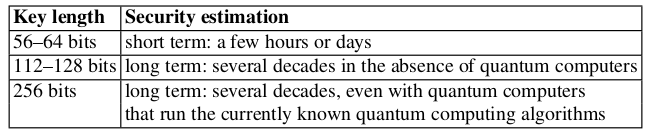
\includegraphics[width=0.7\linewidth]{images/1-TTB.png}
\end{figure}
\section{Some ciphers}
\subsection{Mono-alphabetic substitution}
The mono-alphabetic cipher consists in replacing each letter of the message by a corresponding letter in a mixed alphabet chosen randomly. So we define a substitution table, and we apply our mapping. Let's break it down a little bit.
\begin{itemize}
    \item It is a symmetric scheme.
    \item The key space is $s = 26! > 4\cdot 10 ^{26}$ : a brute-force attack would take some time.
    \item It is breakable using a statistical approach.
\end{itemize}
\begin{center}
    \includegraphics[page=10, width=0.49\textwidth]{Slides/1-Historical-Principles.pdf}
    \includegraphics[page=11, width=0.49\textwidth]{Slides/1-Historical-Principles.pdf}
\end{center}

\subsection{Poly-alphabetic substitution}
Instead of encrypting a entire message with the same mapping, we here divide the message into $t$ blocks.
$$ x = x_1 \Vert x_2 \Vert \dots \Vert x_t$$
Then, we define a mapping for each block. This will be encoded in the key $k$ of the scheme. Indeed, each $k\in K$ will define a \textbf{set of permutations} 
$$k \Rightarrow (p_1, p_2, \dots, p_t) \; .$$
Hence, $E_k(x)$ will be given by 
$$E_k(x) = p_1(x_1) \Vert p_2(x_2) \Vert \dots \Vert p_t(x_t) \Vert $$

As for the decryption key $k'$, it needs to define the set of the $t$ corresponding inverse permutations :

$$k' \Rightarrow (p_1^{-1}, p_2^{-1}, \dots, p_t^{-1}) \; .$$

\subsection{Vigenère cipher} 
\begin{itemize}
    \item Message $m$ of length $|m|$, chosen in $(\mathbb{Z}_{26})^\star$
    \item Key space $K \subset (\mathbb{Z}_{26})^t$. Size : logically $26^t$
    \item Key $k$ taken randomly in $K$, so 
    $$k = (k_0, k_1, \dots, k_{t-1}) \in K$$
\end{itemize}
Then, the encryption of $m$ will result in the concatenation of the XORing of each bit $m_i$ with a part of the key that. Remember that the key has only $t$ parts, so we will repeat the same parts if the message is very long !
$$E_k(m) \equiv E_k(m_0 \Vert m_1 \Vert \dots \Vert m_{|m|-1}) =  \underset{\scriptscriptstyle{0\leq i \leq |m|-1}}{\Vert} (m_i + k_{i  \mod{t}})$$

In practice, the key can actually be a $t$-long string. During the process, each character is converted to a number.

\begin{center}
    \includegraphics[width=0.8\linewidth, page=15]{Slides/1-Historical-Principles.pdf}
\end{center}

\subsubsection{Cryptanalysis of Vigenère cipher}
We stick to Kerckhoff's principles : so we know how every message is encrypted, and the only thing that is kept secret is the key $k$. We don't even know its length $t$. And as it has been seen before, some bits of $m$ are encoded with the same key chunk because of the modulo in the XOR ($k_{i\mod t})$. So we can group the bits of $m$ that are encoded with the same chunks.

$$m_i, m_{i+ t}, m_{i+2t} \longleftarrow k_{i\mod t}$$

For each 
\end{document}